\documentclass[11pt]{article}

\usepackage[margin=1in]{geometry}
\usepackage{amsmath, amssymb}
\usepackage{booktabs}
\usepackage{graphicx}
\usepackage{hyperref}
\usepackage{xcolor}
\usepackage{listings}

\graphicspath{{figures/}}

\lstdefinestyle{commands}{
  basicstyle=\ttfamily\small,
  breaklines=true,
  frame=single,
  backgroundcolor=\color{gray!8}
}

\title{Maximum Independent Set: Computational Project}
\author{}
\date{}

\begin{document}

\maketitle

\section{Problem}

We compare greedy and integer-programming methods for maximum independent set on
Erdos--Renyi graphs $G(n,d/n)$ and on a real SNAP network.

For a graph $G=(V,E)$, the integer-programming formulation is
\begin{align*}
\max \quad & \sum_{i \in V} x_i \\
\text{s.t.} \quad & x_u + x_v \leq 1 && \text{for every edge } (u,v) \in E, \\
& x_i \in \{0,1\} && \text{for every vertex } i \in V.
\end{align*}
Here $x_i=1$ means vertex $i$ is included in the independent set.

For $G(n,d/n)$, the asymptotic reference values are
\[
\text{greedy scale} = \frac{\log d}{d}n,
\qquad
\text{optimum scale} = \frac{2\log d}{d}n.
\]
For $d=20$, these are approximately $0.1498n$ and $0.2996n$.

\section{Algorithms}

The greedy baseline repeats random-order greedy and also tries a minimum-degree
greedy heuristic, keeping the largest feasible independent set found. In the
random-order method, vertices are shuffled, and a vertex is added if none of its
neighbors has already been selected.

The IP model uses one binary variable per vertex and one edge constraint per
edge. It is solved with SciPy's MILP interface to HiGHS. For each run we record
the incumbent size, solver status, runtime, best bound, and MIP gap.

\section{Erdos--Renyi Starter Results}

The starter experiment used $d=20$, seeds $0,1,2$, and a 30-second IP time
limit.

\begin{lstlisting}[style=commands]
scripts/run_er_d20_starter.sh
\end{lstlisting}

The raw results are in \texttt{results/er\_d20\_starter\_results.csv}. The plot
in Figure~\ref{fig:er-starter} compares greedy, IP incumbents, and the two
theoretical reference fractions.

\begin{figure}[htbp]
  \centering
  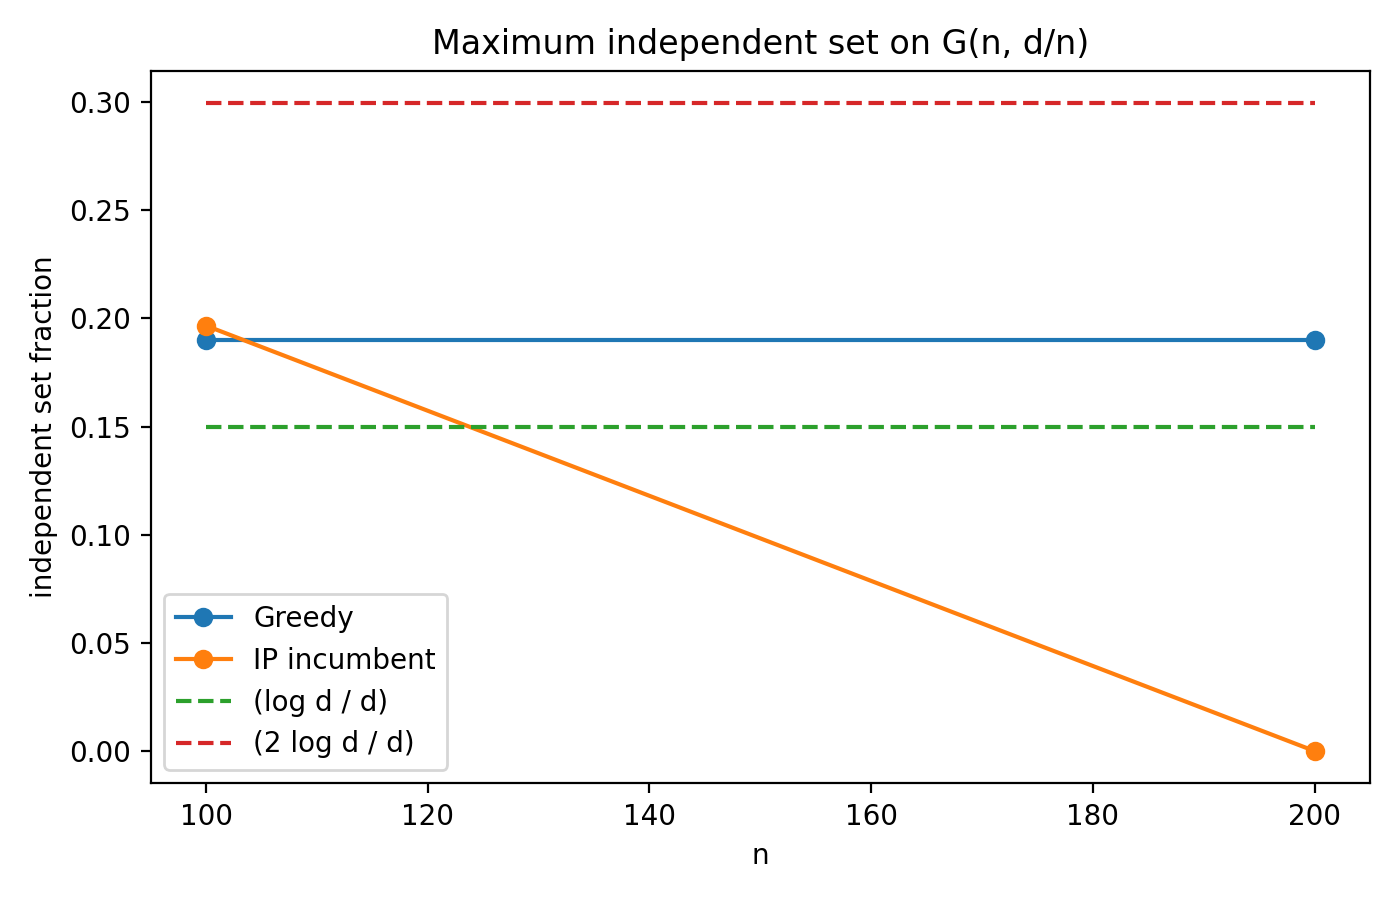
\includegraphics[width=0.78\linewidth]{er_d20_starter_fraction.png}
  \caption{Independent set fraction on $G(n,20/n)$ for the starter ER runs.}
  \label{fig:er-starter}
\end{figure}

\begin{table}[htbp]
\centering
\caption{Starter results for $G(n,20/n)$ over seeds $0,1,2$.}
\label{tab:er-starter}
\begin{tabular}{rllll}
\toprule
$n$ & Greedy sizes & IP sizes/status & $(\log d/d)n$ & $(2\log d/d)n$ \\
\midrule
100 & 18, 19, 20 & 20, 19, 20; all optimal & 14.98 & 29.96 \\
200 & 39, 36, 39 & no incumbent returned in 30s & 29.96 & 59.91 \\
\bottomrule
\end{tabular}
\end{table}

For $n=100$, IP proves optimality quickly and beats the greedy threshold. For
$n=200$, the SciPy/HiGHS IP run hit the 30-second time limit before returning an
incumbent, while greedy still found sets well above $(\log d/d)n$.

\section{SNAP Result: ca-GrQc}

The real-network experiment used the SNAP \texttt{ca-GrQc} collaboration graph.
The command was
\begin{lstlisting}[style=commands]
scripts/run_ca_grqc.sh
\end{lstlisting}
The raw results are in \texttt{results/ca\_grqc\_results.csv}.

\begin{table}[htbp]
\centering
\caption{SNAP dataset statistics.}
\label{tab:snap-stats}
\begin{tabular}{lrrrrr}
\toprule
Dataset & $n$ & $m$ & Avg. degree & Components & Largest component \\
\midrule
ca-GrQc & 5241 & 14484 & 5.527 & 354 & 4158 \\
\bottomrule
\end{tabular}
\end{table}

\begin{table}[htbp]
\centering
\caption{Algorithm results on \texttt{ca-GrQc}.}
\label{tab:snap-results}
\begin{tabular}{lrrl}
\toprule
Method & Independent set size & Runtime & Status \\
\midrule
Repeated greedy & 2458 & 1.80s & feasible \\
IP & 2458 & 0.38s & optimal \\
\bottomrule
\end{tabular}
\end{table}

\begin{figure}[htbp]
  \centering
  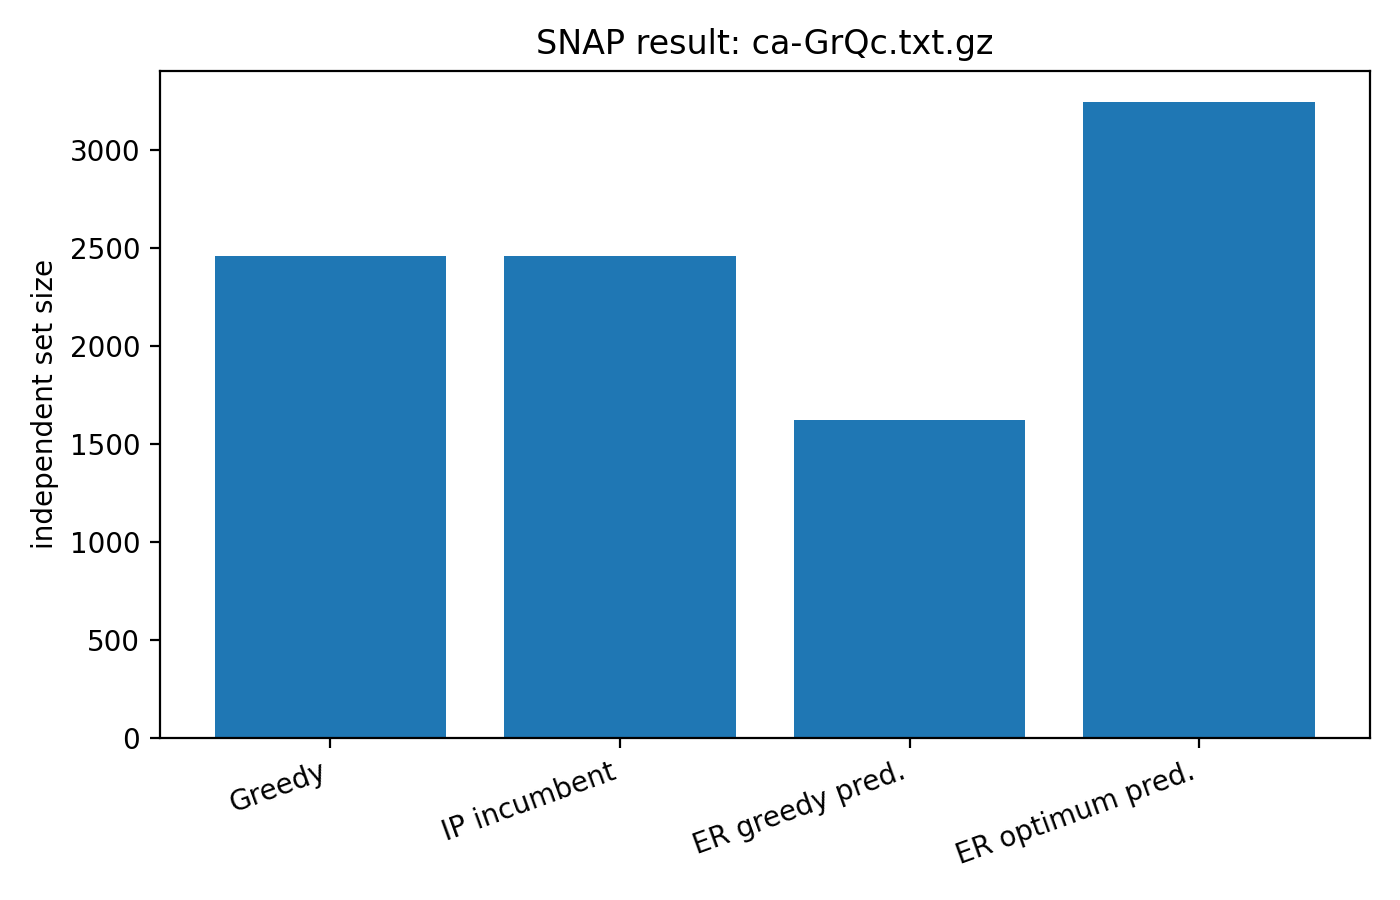
\includegraphics[width=0.72\linewidth]{ca_grqc_comparison.png}
  \caption{Greedy, IP, and ER-style predictions for \texttt{ca-GrQc}.}
  \label{fig:ca-grqc}
\end{figure}

The ER prediction using the average degree gives approximately 1621 for the
greedy scale and 3242 for the asymptotic optimum scale. The actual optimum of
2458 lies between these two values. This is not surprising: \texttt{ca-GrQc} is
a real collaboration network with many components and non-ER structure, so
average degree alone is not enough to predict the independent-set size.

\section{Next Experiments}

The next step is to use longer IP limits for $n=200$ and then try
$n=500,1000,2000$:
\begin{lstlisting}[style=commands]
PYTHONPATH=src python3 -m mis_project.experiments er \
  --d 20 \
  --n-values 200 500 1000 \
  --seeds 0 1 2 \
  --greedy-repeats 100 \
  --time-limit 300 \
  --output results/er_d20_larger_results.csv
\end{lstlisting}

The final writeup should emphasize when IP proves optimality, when it only finds
an incumbent, and when it fails to return an incumbent before the time limit.

\section{Conclusion}

The starter runs show that IP can prove optimality on small random graphs, but
the difficulty increases quickly as $n$ grows. Greedy is extremely fast and
already beats the $(\log d/d)n$ threshold in the tested $d=20$ instances. On the
real \texttt{ca-GrQc} network, greedy found an optimal solution, and the IP
solver proved optimality quickly. The real-network result also shows that the
Erdos--Renyi prediction based only on average degree is only a rough reference,
not an accurate model for structured networks.

\end{document}
